\PassOptionsToPackage{pdfpagelabels=false}{hyperref}
\documentclass[fleqn,usenatbib,usedcolumn]{mnras}
%==============================================================================%
\usepackage[british]{babel}             % British English hyphenation
\usepackage{txfonts}                  % Good fonts
% Use vector fonts, so it zooms properly in on-screen viewing software
% Don't change these lines unless you know what you are doing
%\usepackage[T1]{fontenc}
%\usepackage{ae,aecompl}
%%%%% AUTHORS - PLACE YOUR OWN PACKAGES HERE %%%%%
\usepackage{graphicx}	% Including figure files
\usepackage{hyperref} % hyperlinks
\usepackage{natbib}
\usepackage{aastexmacros}
\usepackage{tikz}
\usepackage[caption=false]{subfig}
\usepackage[mediumspace,mediumqspace,Grey,squaren]{SIunits}
%%%%%%%%%%%%%%%%%%%%%%%%%%%%%%%%%%%%%%%%%%%%%%%%%%

%%%%% AUTHORS - PLACE YOUR OWN COMMANDS HERE %%%%%
\usetikzlibrary{shapes,arrows,calc,positioning}

\renewcommand{\vec}[1]{\mathbf{#1}}
% \newcommand{\text}{\mathrm}
\newcommand{\jansky}{\text{Jy}}
\newcommand{\cheng}[1]{ {\color{teal}[{\bf Cheng:~{#1}}]} }
\newcommand{\matthew}[2]{ {\color{white!20!violet}[{\bf TODO(#1):~{#2}}]} }
\newcommand{\todo}[1]{ {\color{red}[{\bf TODO:~{#1}}]} }

%%%%%%%%%%%%%%%%%%%%%%%%%%%%%%%%%%%%%%%%%%%%%%%%%%

%%%%%%%%%%%%%%%%%%% TITLE PAGE %%%%%%%%%%%%%%%%%%%

\title[ML CDFS]{Radio Galaxy Zoo: Machine learning methods for radio source host galaxy cross-identification}

\author[RGZ ML Team]{M. J. Alger$^{1}$, J. K. Banfield$^{1, 2, 3}$, C. S. Ong$^{4, 5}$, O. I. Wong$^{2, 6}$, others
\\
% List of institutions
$^{1}$Research School of Astronomy and Astrophysics, The Australian National University, Canberra, ACT 2611, Australia\\
$^{2}$ARC Centre of Excellence for All-Sky Astrophysics (CAASTRO)\\
$^{3}$Western Sydney University, Locked Bag 1797, Penrith South, NSW 1797, Australia\\
$^{4}$Data61, CSIRO, 7 London Circuit, Canberra ACT 2601, Australia\\
$^{5}$Research School of Computer Science, The Australian National University, Canberra, ACT 2601, Australia\\
$^{6}$International Centre for Radio Astronomy Research-M468, The University of Western Australia, 35 Stirling Hwy, Crawley, WA 6009, Australia
}

% These dates will be filled out by the publisher
\date{Accepted XXX. Received XXX}

% Enter the current year, for the copyright statements etc.
\pubyear{2017}

% Don't change these lines
\begin{document}
\label{firstpage}
\pagerange{\pageref{firstpage}--\pageref{lastpage}}
\maketitle

% Abstract of the paper
\begin{abstract}
  We present a machine learning approach for the task of determining the
  infrared host galaxies of radio emissions detected in wide-area radio surveys.
  Training a machine learning algorithm requires a large amount of labelled
  training data, which can be difficult or expensive to acquire. Radio Galaxy
  Zoo, a citizen science project on the Zooniverse platform, provides a large
  number of radio host cross-identifications which may be used as labels for
  training. We find that while machine learning algorithms trained on expert
  labels outperform those trained on the crowdsourced Radio Galaxy Zoo labels,
  the accuracies are comparable and the crowdsourced labels are still useful for
  training. \matthew{Julie}{Rewrite.}
\end{abstract}

% Select between one and six entries from the list of approved keywords.
% Don't make up new ones.
\begin{keywords}
galaxies: active -- galaxies: clusters -- radio continuum: galaxies
\end{keywords}

%%%%%%%%%%%%%%%%%%%%%%%%%%%%%%%%%%%%%%%%%%%%%%%%%%
%%%%%%%%%%%%%%%%% BODY OF PAPER %%%%%%%%%%%%%%%%%%

\section{Introduction}\label{introduction}

  Next generation radio telescopes such as the Australian SKA Pathfinder
  \citep[ASKAP;][]{johnston07} and Apertif \citep{verheijen08} will conduct
  increasingly wide, deep, and high-resolution radio surveys, producing large
  amounts of data. The Evolutionary Map of the Universe survey
  \citep[EMU;][]{norris11} using ASKAP and the WODAN survey \citep{rottgering11}
  using Apertif are expected to detect over 100 million radio components between
  them, compared to the 2.5 million radio components already known
  \citep{banfield15}.

  An important part of processing this data is cross-identifying observed radio
  emission regions with observations of their host galaxy in surveys at other
  wavelengths. Radio host cross-identification is a difficult task. While
  pointlike or compact sources of radio emission usually coincide with the host
  galaxy, a large proportion of radio sources are considerably more complex.
  Radio emissions from radio-loud active galactic nuclei (AGN) may be
  complicated structures not clearly related to the host galaxy, and are often
  composed of multiple, separate components. These AGN are expected to dominate
  approximately 30\% of sources detected by EMU \citep{norris11}. Small surveys
  of a few thousand sources such as the Australia Telescope Large Area Survey
  \citep[ATLAS;][]{norris06,middelberg08} can be cross-identified manually, but
  this is impractical for larger surveys.

  One approach to cross-identification is crowdsourcing, where members of the
  public volunteer to cross-identify radio emissions (sources) with their host
  galaxies. This is the premise of Radio Galaxy Zoo \citep[RGZ;][]{banfield15},
  a citizen science project hosted on the highly successful Zooniverse platform
  \citep{lintott08}. Volunteers are shown images of the radio sky, and are asked
  to identify the radio sources in each image \matthew{Julie}{Is this sentence
  unambiguous enough?}. They are then asked to cross-identify each radio source
  with its host galaxy in a corresponding infrared image. Radio Galaxy Zoo
  provides a large dataset of 100~267 radio host cross-identifications and radio
  source morphologies \citep{wong17}. While this is a much larger number of
  cross-identifications than have been made by experts, it is still far short of
  the millions of radio sources expected to be detected in upcoming radio
  surveys.

  Automated algorithms have been developed for this cross-identification
  problem. \citet{fan15} developed a method of cross-identification using
  Bayesian hypothesis testing, fitting a three-component model to extended radio
  sources under the assumption that radio sources are composed of a core radio
  component and two lobe components. The core radio component is coincident with
  the host galaxy, so cross-identification amounts to finding the galaxy
  coincident with the core in the most likely model fit. This method is easily
  extended to use other, more complex models, but it is purely geometric and
  does not incorporate other information such as the properties of the potential
  host galaxy. Additionally, there may be new classes of radio sources detected
  in future surveys like EMU which do not fit the model. \citet{weston17}
  developed a modification of the likelihood ratio method of
  cross-identification \citep{richter75likelihood} for application to EMU.
  However, this method is only intended to cross-identify `simple' sources
  consisting of a single, isolated radio component \citep{norris17unexpected}.
  \matthew{Julie}{Can you elaborate on this?}

  In order to investigate methods for efficiently and effectively classifying
  radio galaxy hosts for upcoming large radio surveys, we have developed a
  machine learning approach for radio host cross-identification using standard
  machine learning techniques. In \autoref{sec:data} we describe the data we
  used to train our methods. In \autoref{sec:method} we describe how we cast the
  radio host galaxy cross-identification problem as a standard machine learning
  problem. In \autoref{sec:results} we present results of applying our method to
  the \emph{Chandra} Deep Field - South (CDFS) and in \autoref{sec:elais} we
  apply the cross-identifiers trained on CDFS to the ESO Large Area ISO Survey -
  South 1 (ELAIS-S1) field.

  \begin{figure}
    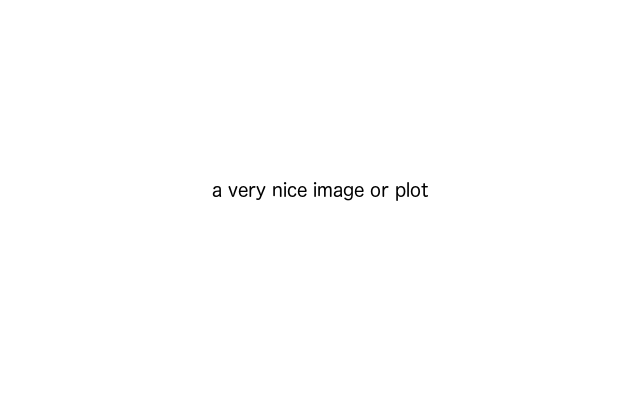
\includegraphics[width=\linewidth]{images/placeholder.png}
    \caption{\matthew{Julie}{Define component, source, primary component, host, in a figure.}}
  \end{figure}

\section{Data}\label{sec:data}
    
  We use data from the citizen science project Radio Galaxy Zoo
  \citep{banfield15}, the Australia Telescope Large Area Survey
  \citep[ATLAS;][]{franzen15}, and the \emph{Spitzer} Wide-area Infrared
  Extragalactic survey \citep[SWIRE;][]{lonsdale03swire, surace05swire}.

  \subsection{ATLAS}\label{sec:atlas}

    ATLAS \citep{franzen15} is a wide-area radio survey of the CDFS and ELAIS-S1
    fields at 1.4 GHz. ATLAS has a sensitivity of
    \unit{14}{\micro\jansky} on CDFS and \unit{17}{\micro\jansky} on ELAIS-S1.
    CDFS covers 3.6~deg$^2$ and contains 3034 radio components above 5$\sigma$.
    ELAIS-S1 covers 2.7~deg$^2$ and contains 2084 radio components above
    5$\sigma$ \citep{franzen15}.

    ATLAS is a pilot survey for the EMU \citep{norris11} survey, which will
    cover the entire southern sky and is expected to detect approximately 70
    million new radio sources. EMU will be conducted at the same depth and
    resolution as ATLAS, so methods developed for processing ATLAS data are
    expected to work for EMU.

    \begin{table}
      \caption{Catalogues of ATLAS/SWIRE cross-identifications for the CDFS
        and ELAIS-S1 fields. The method used to generate each catalogue is
        shown, along with the number of radio components cross-identified in each
        field.}
      \label{tab:atlas-cids}
      \begin{tabular}{ll|cc}
        \hline
        Catalogue & Method & \#CDFS & \#ELAIS-S1\\
        \hline
        \citet{norris06} & Manual & 784 & 0\\
        \citet{middelberg08} & Manual & 0 & 1366\\
        \citet{fan15} & Bayesian models & 784 & 0\\
        \citet{wong17} & Crowdsourcing & 2460 & 0 \\
        \citet{weston17} & Likelihood ratio & 3078 & 2113\\
        \hline
      \end{tabular}
    \end{table}

    A number of catalogues have been produced cross-identifying radio components
    in ATLAS with host galaxies in SWIRE. These catalogues are summarised in
    \autoref{tab:atlas-cids}.

    % \citet{norris06} produced a catalogue of cross-identifications of 784
    % radio sources with their infrared counterparts in SWIRE.
    % \citet{middelberg08} produced a catalogue of cross-identifications of
    % {[}NNNN{]} radio sources with their infrared counterparts in SWIRE.
    % {[}TODO: Make this less clunky and talk about Fan et al.{]}

    % Radio Galaxy Zoo (\autoref{sec:rgz}) produced a catalogue of
    % crowdsourced cross-identifications of 2460 ATLAS radio objects in CDFS
    % \citep{wong17}.
    % % As these cross-identifications have been based on
    % % volunteer classifications, this catalogue is expected to be less accurate
    % % than an expert catalogue like that produced by \citet{norris06}.

  \subsection{SWIRE}\label{sec:swire}

    SWIRE \citep{lonsdale03swire, surace05swire} is a wide-area infrared survey
    at the four IRAC wavelengths 3.6, 4.5, 5.8, and
    \unit{8.0}{\micro\meter}, with $5\sigma$ noise levels of 7.3,
    9.7, 27.5, and \unit{32.5}{\micro\jansky} respectively
    \citep{lonsdale03swire}. It covers eight fields, including CDFS and ELAIS-S1
    which are also covered by ATLAS. SWIRE is thus the source of infrared
    observations for cross-identification with ATLAS. SWIRE catalogues 221,535
    objects in CDFS and 186,059 objects in ELAIS-S1.

  \subsection{Radio Galaxy Zoo}\label{sec:rgz}

    Radio Galaxy Zoo asks volunteers to cross-identify radio components with
    their infrared host galaxies. There are a total of 177~461 radio components
    in Radio Galaxy Zoo, sourced from ATLAS and Faint Images of the Radio Sky at
    Twenty-Centimeters \citep[FIRST;][]{white97first}. These components are
    cross-identified to host galaxies detected in SWIRE and by the
    \emph{Wide-Field Infrared Survey Explorer} \citep[WISE;][]{wright10wise},
    respectively.

    Volunteers are presented with a random radio image centred on a radio
    component, and a corresponding infrared image centred on the same
    location. The radio image may contain multiple radio components.
    Classification of these images is a two-step process. First, volunteers
    select which radio components are part of the same radio source. Second,
    volunteers associate each radio source with a host galaxy visible in the
    infrared image. A more detailed description can be found in
    \citet{banfield15}.

    To reduce noise in the classification, each radio component is shown to
    multiple volunteers. Compact radio components are shown to 5 volunteers,
    while extended radio components are shown to 20 volunteers. Once a radio
    object has been classified by the required number of volunteers, it is
    considered `complete'. Complete classifications are combined to produce
    the final catalogue of Radio Galaxy Zoo source component counts and
    cross-identifications. The most commonly chosen associations of radio
    components to radio sources are chosen as the radio morphology
    classification for the image. The host galaxy locations selected by
    volunteers who agreed with the most common radio morphology classification
    are combined by maximising over a kernel density estimate of the locations.
    These locations are then matched to the nearest SWIRE object within
    3~arcsec. A full description of the catalogue generation can be found in
    \citet{wong17}. As of 30 March 2016, there are 97~807 complete
    classifications of FIRST components, and 2460 complete classifications of
    ATLAS CDFS components.

    In this paper we focus on the Radio Galaxy Zoo cross-identifications of
    the ATLAS~CDFS and SWIRE surveys. There are two main reasons for this. The
    first is that ATLAS is the pilot study for EMU where automated methods
    like ours will be used. The second is that ATLAS is composed of two
    fields, so we can train methods on one field and test these methods on
    the other field to ensure that our methods apply in different areas of
    the sky observed by the same telescope.

    \matthew{Julie}{Explain what components went into RGZ.} Each primary
    component found in the ATLAS DR3 component catalogue appears in Radio Galaxy
    Zoo. Non-primary components may appear within the image of a primary
    component, but do not have their own entry in Radio Galaxy Zoo. We will
    henceforth only discuss the primary components. For ATLAS components, the
    radio and infrared images shown to volunteers are $2 \times 2$~arcmin.

  \section{Method}\label{sec:method}

  \subsection{Cross-identification as binary
  classification}\label{cross-identification-as-binary-classification}

    We focus on the problem of host galaxy cross-identification without
    reference to radio morphology. Given a radio component, we want to find the
    corresponding host galaxy as a citizen scientist would using Radio Galaxy
    Zoo. The input is thus a radio image and an infrared image with a given
    radius. We choose a radius of 1~arcmin to match Radio Galaxy Zoo, which uses
    $2 \times 2$~arcmin cutouts of ATLAS images. We make the assumption that
    each radio image represents a single, complex extended source. This is not
    the case in general and a radio image may contain many different radio
    sources with unique host galaxies. If we had access to radio morphology
    information, we could use this to isolate relevant components and hence more
    accurately cross-identify sources, but this is outside the scope of this
    paper. We also note that this assumption will bias our results against radio
    emission that extends beyond the 1~arcmin cutout size, however, these are
    uncommon in ATLAS with 9 radio sources identified by \citet{norris06} as
    having components further than 1~arcmin apart (and of these, 5 are in Radio
    Galaxy Zoo). The radio cross-identification task then amounts to locating
    the host galaxy within the associated radio and infrared images. This is
    formalised as an object localisation problem: Given a radio image and an
    infrared image centred on a radio component, locate the host galaxy of the
    radio component.    % S031, S336, S081, S576, S136, S719, S618, S707, S287
    % ARG0003r2r, -, -, ARG0003r5h, ARG0003r2d, -, ARG0003r1s, -, ARG0003r8q

    \begin{figure}
      \centering
      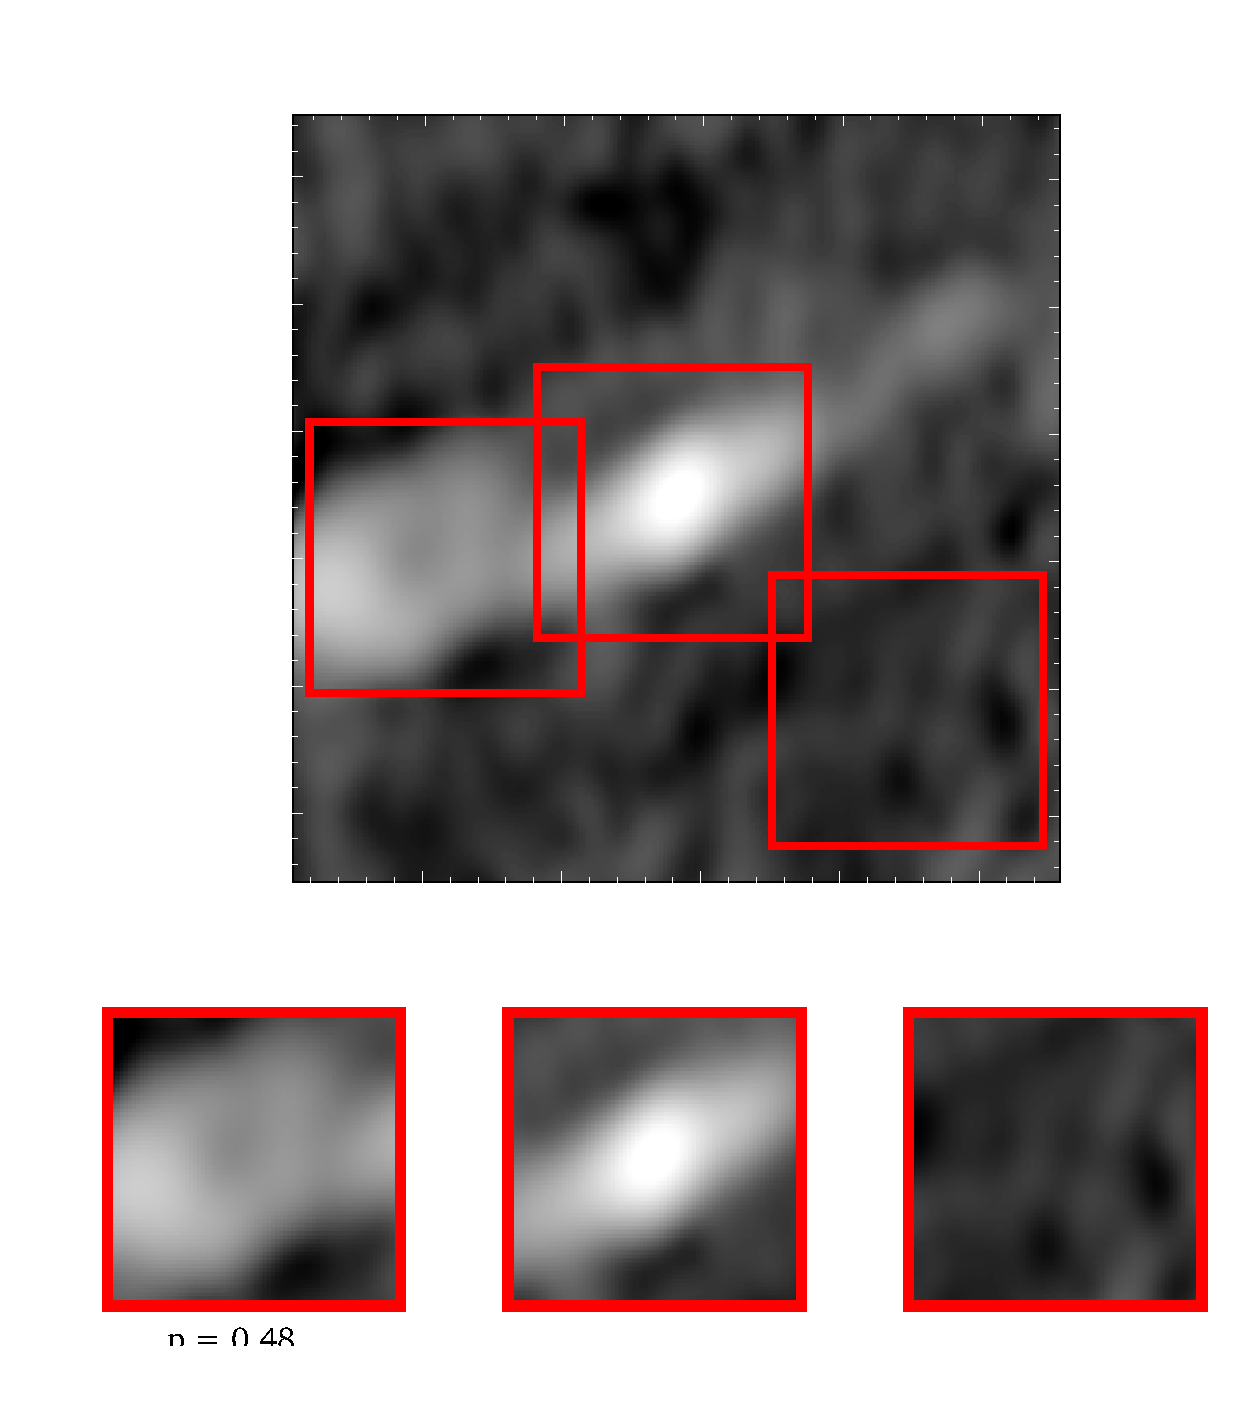
\includegraphics[width=0.8\columnwidth]{images/elais_0093C1_with_boxes}
      \caption{An example of localising the host galaxy of a radio source using
        our method. This image is from ATLAS and is centred on $\alpha =
        00^\text{h}33^\text{m}06.36^\text{s}, \delta = -43^\circ{}10'30.1''$. Boxes
        represent $32 \times 32$ pixel windows centred on various locations in
        the image. The corresponding image patches from each window are shown
        beneath. The image patch of each window represents the location the
        window is centred on. The probabilities of each patch coinciding with
        the host galaxy would then be estimated by a classification model. The
        probabilities shown are for illustration only. In this example, the
        centre window of the image would be chosen as the location of the host
        galaxy, as the window centred on it has the highest probability.}
      \label{fig:windows}
    \end{figure}

    A common approach to object localisation is to estimate the probability
    that each location in the image is coincident with the desired object. In
    practice this amounts to taking fixed-size windows of the image centred on
    each pixel and estimating the probability that each window is centred on
    the object. The location associated with the highest probability window is
    then assumed to be the location of the object. Applying this to radio host
    cross-identification, we consider windows of a radio/infrared image and
    estimate the probability that each window is centred on the host galaxy.
    This approach is illustrated in \autoref{fig:windows}.
    In computer vision a sliding window is commonly used: every possible patch
    in the image is considered.

    This task can be made more efficient if we have a prior on the location of
    the object we are localising. For our prior, we assume that the host galaxy
    is always visible in the infrared and thus we only need consider windows
    centred on infrared sources. This assumption usually holds, except for a
    rare class of infrared-faint radio sources. \citet{norris06} found 22 such
    radio sources in their sample of 784 bright ATLAS components in CDFS. This
    leads us to a binary classification task: Given an infrared source, compute
    the probability that it is a host galaxy. To find the host galaxy given a
    radio source, classify each galaxy within 1~arcmin of the source and select
    the galaxy with the highest probability of being a host galaxy. This is a
    good formulation as binary classification is a very common problem in
    machine learning and there are many different methods readily available to
    solve it.

    % \cheng{Be careful about the difference between a binary classifier and
    % a class probability estimator. $\mathcal{Y}$ can be binary or in the unit
    % interval.}
    Solving the radio cross-identification task amounts to modelling a function
    $f$ from infrared sources $\mathcal{X}$ to the probability that an infrared
    source belongs to a binary class in $\mathcal{Y} = \{0, 1\}$:
    \begin{equation}
        f(x) \coloneqq \text{Pr}\left(\mathcal{Y} = 1 \mid \mathcal X = x\right).
    \end{equation}
    The space of infrared sources $\mathcal{X}$ needs to be encoded as a vector
    for the models we will use. We describe this in
    \autoref{vector-representation-of-infrared-sources}. There are many options
    for modelling $f$. In this paper we apply three different models: logistic
    regression, random forests, and convolutional neural networks.

    \begin{figure}
      \centering
      % http://www.texample.net/tikz/examples/simple-flow-chart/
      \tikzstyle{decision} = [diamond, draw, fill=white,
          text width=4.5em, text badly centered, inner sep=0pt]
      \tikzstyle{block} = [rectangle, draw, fill=white,
          text width=5em, text centered, rounded corners, minimum height=4em]
      \tikzstyle{line} = [draw, -latex']
      \begin{tikzpicture}[node distance=6mm, auto]
        \node [block] (init) {input radio source};
        \node [decision, right= of init] (iscompact) {compact?};
        \node [block, below= of iscompact] (compact) {find nearest infrared object};
        \node [block, right= of iscompact] (resolved) {find nearby infrared objects};
        \node [block, fill=black!10, right= of resolved] (classify) {classify objects};
        \node [block, below= of classify] (best) {find highest probability object};
        \coordinate (middle) at ($(compact)!0.5!(best)$);
        \node [block, below= of middle, fill=green!10] (done) {\textbf{host galaxy}};
        \path [line] (init) -- (iscompact);
        \path [line] (iscompact) -- (compact) node [midway] {yes};
        \path [line] (compact) -- (done);
        \path [line] (iscompact) -- (resolved) node [midway] {no};
        \path [line] (resolved) -- (classify);
        \path [line] (classify) -- (best);
        \path [line] (best) -- (done);
      \end{tikzpicture}
      \caption{A cross-identification method employing a binary classifier. As
        input we accept a radio source. If the source is compact, we select
        the nearest infrared object as the host galaxy. If the source is
        resolved, we classify all infrared objects nearby within radius $R$
        and select the highest probability object as the host galaxy. The grey
        box is the classifier, which can be any binary classifier that outputs
        a probability.}
      \label{fig:flowchart}
    \end{figure}

    We can improve upon this cross-identification method by filtering out
    compact radio sources, which are much easier to cross-identify --- the
    nearest SWIRE object may be identified as the host galaxy, or a more
    complex method such as likelihood ratios may be applied
    \citep[see][]{weston17}. A full cross-identification pipeline making use
    of this alongside a binary classifier is shown in \autoref{fig:flowchart}.

  \subsection{Limitations of our approach}
  \label{sec:limitations}

    Our assumptions are:
    \begin{itemize}
      \item A radio image represents a single radio source and contains exactly
        one host galaxy.
      \item The host galaxy of a radio component is within 1~arcmin of the
        component.
      \item The host galaxy appears in the SWIRE catalogue.
    \end{itemize}

    \begin{figure}
      \centering
      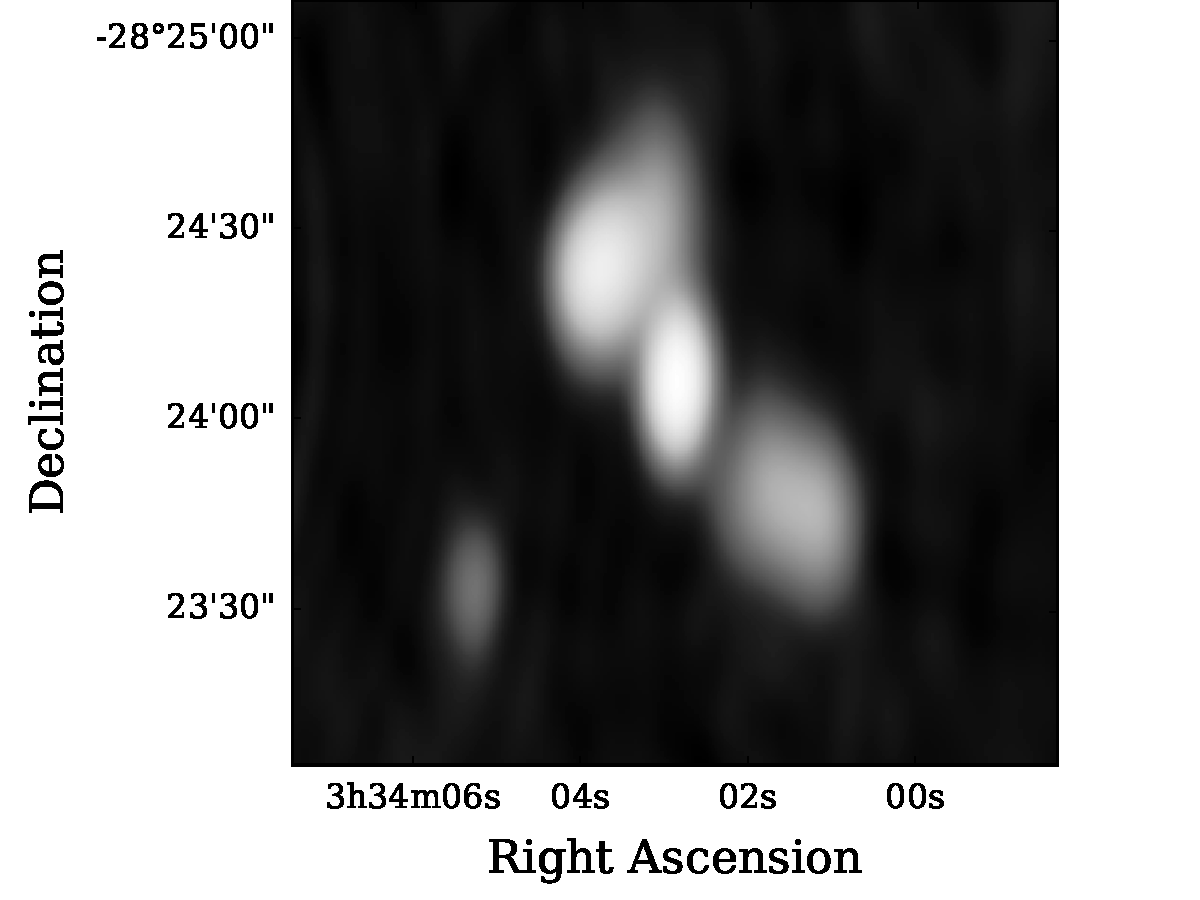
\includegraphics[width=\linewidth]{images/ARG0003r2v_radio.pdf}
      \caption{$2'$-wide radio image centred on ATLAS3\textunderscore{}J033402.87-282405.8C.
        %(ARG0003r2v)
        This radio source breaks our assumption that there are no other radio
        sources within 1~arcmin of the source. Another radio source is visible
        to the upper-left. Host galaxies found by Radio Galaxy Zoo volunteers
        are shown by a cross.}
      \label{fig:broken-isolation}
    \end{figure}

    \begin{figure}
      \centering
      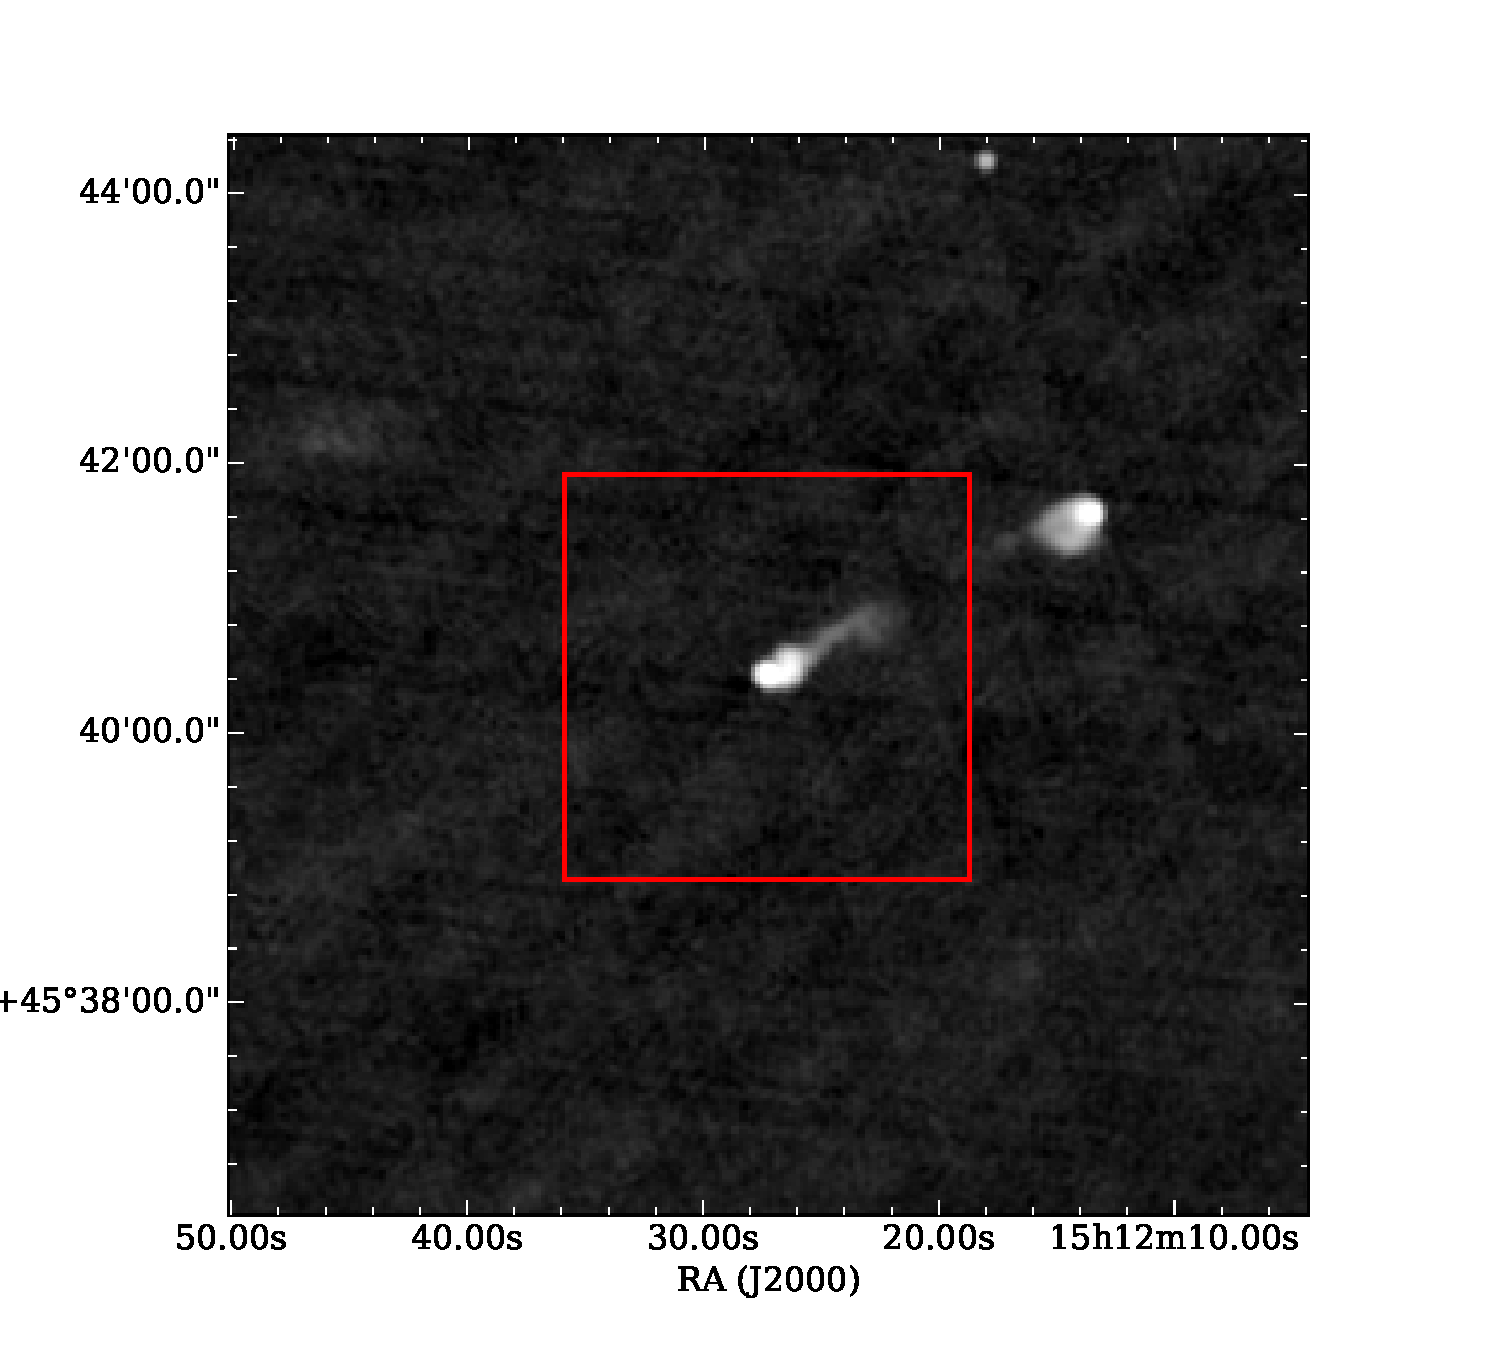
\includegraphics[width=\linewidth]{images/ARG0000u0h_first_8.pdf}
      \caption{A $8'$-wide radio image from FIRST, centred on
        FIRSTJ151227.2+454026. The $3'$-wide red box indicates the boundaries of
        the image of this radio component shown to volunteers in Radio Galaxy
        Zoo. This radio source breaks our assumption that the whole radio source
        is visible in the chosen radius. As one of the lobes of the radio source
        is outside of the image, a volunteer (or automated algorithm) looking at
        the $3'$-wide image may be unable to determine that this is a radio
        double or locate the host galaxy.}
      \label{fig:broken-contains}
    \end{figure}

    The key problem with this approach is our assumption that the radio sky
    within 1~arcmin radius contains only one, complete radio source. The problem
    is two-fold: This radius may contain multiple sources, or it may not contain
    the entirety of the source. If the radius contains multiple sources then
    there will also be multiple hosts in our input images (which breaks our
    assumption that there is only one); even a perfect classifier can only
    accurately cross-identify \emph{one} host in an image with multiple. An
    example of a radio source that breaks the assumption in this way is shown in
    \autoref{fig:broken-isolation}. If the radius does not contain the whole
    source, then we are missing radio information useful for finding the host
    galaxy. This is a difficult problem even for non-automated methods as radio
    sources can be extremely wide --- for example, Radio Galaxy Zoo found a
    radio giant that spanned over three different images presented to volunteers
    and the full source was only cross-identified by the efforts of citizen
    scientists \citep{banfield15}. An example of a radio image where part of the
    radio source is outside the search radius is shown in
    \autoref{fig:broken-contains}. The problems are in opposition to each other:
    To reduce the number of sources in an input image, we can reduce the image
    radius, but this increases the chance that we will miss relevant radio
    source information, and vice versa.

    Our assumptions impose an upper bound on how well we can cross-identify
    radio sources, which can be estimated by considering how accurately a
    \emph{perfect} binary classifier cross-identifies radio sources under our
    method. Using the expert labels (\autoref{labels}) to classify SWIRE objects
    to 100~percent accuracy on the binary classification task results in a
    cross-identification accuracy of $(96.74 \pm 1.76)$~percent across the four
    CDFS quadrants under our assumptions, which we take as an upper bound on our
    cross-identification accuracy.

    \begin{figure}
      \centering
      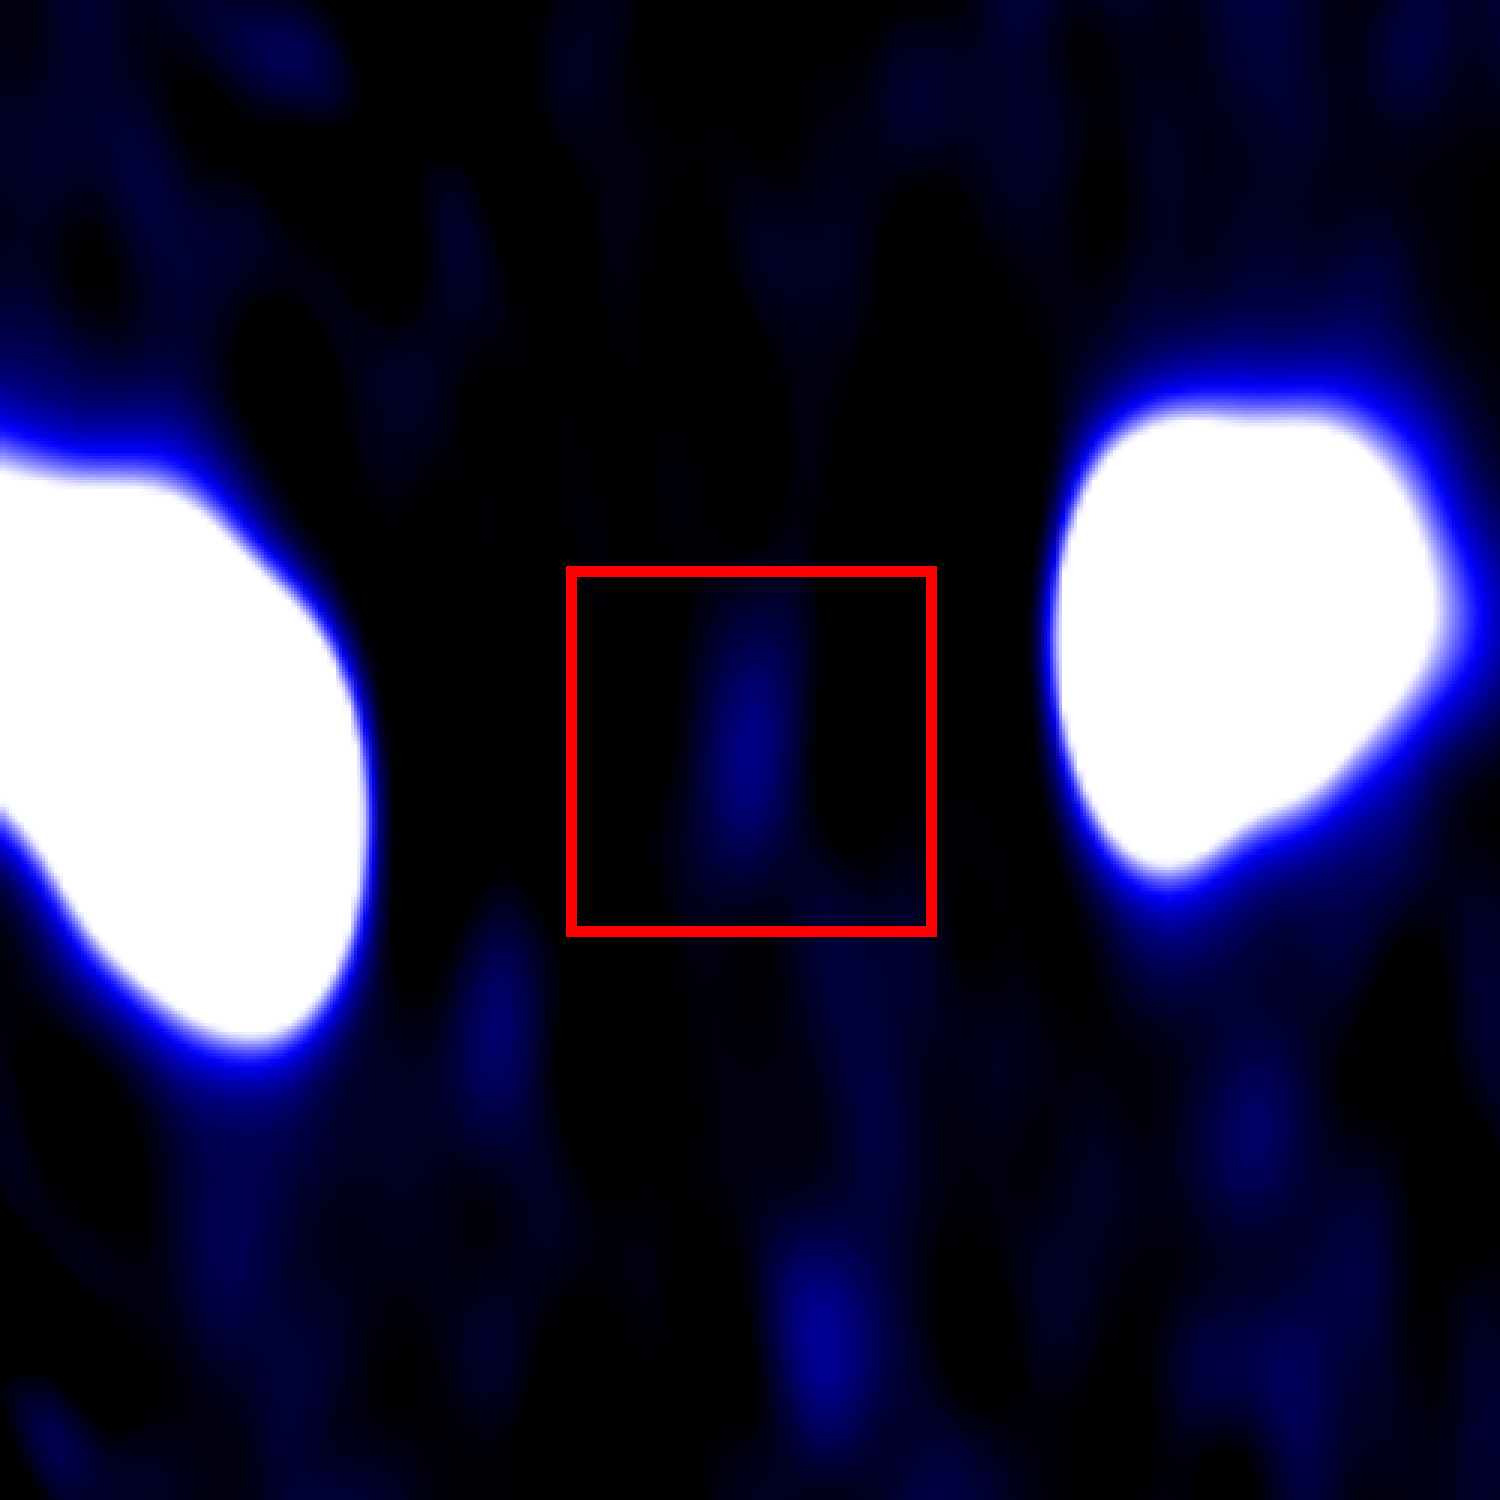
\includegraphics[width=\linewidth]{images/ARG0003sky_radio}
      \caption{A radio image centred on $\alpha =
        03^\text{h}26^\text{m}39.12^\text{s}$, $\delta = -28^\circ{}07'58.80''$.        %ARG0003sky
        This is an example of a radio source where the window centred on the
        host galaxy, shown as a rectangle, does not contain enough radio
        information to correctly identify the galaxy as the host.}
      \label{fig:broken-window-size}
    \end{figure}

    A related issue is that we need to choose a window size for the image
    representations of each SWIRE object. If this image is too small, radio
    emission may extend past the edges of the window, and it may be impossible
    to identify the galaxy as a host galaxy. If the image is too large, then
    too much information will be included and it will be difficult or
    computationally expensive to classify. We chose a window size of $32
    \times 32$ pixels, shown as a red rectangle in
    \autoref{fig:windows} and \autoref{fig:broken-window-size}.

  \subsection{Feature vector representation of infrared sources}
  \label{vector-representation-of-infrared-sources}

    Most binary classification methods require that the inputs to be classified
    are an array of real values called \emph{feature vectors}. We thus need to
    choose a feature vector representation of our candidate host galaxies.

    Infrared observations of the CDFS field are taken from SWIRE. We use the
    CDFS Fall '05 SWIRE catalogue \citep{surace05swire} to generate candidate
    hosts to classify. Radio observations of the CDFS field are taken from
    ATLAS. As the visual appearance of objects in SWIRE are likely irrelevant to
    whether the galaxy is a host galaxy, the candidate host location encodes
    almost all information we could gain from the infrared image. We therefore
    only use the radio image for object localisation. \matthew{Julie}{How is the
    wording?}

    We represent each candidate host as 1034 real-valued features. For a given
    candidate host, these features are:
    \begin{itemize}
      \item the logarithm of the ratio of fluxes of the candidate host in the
        four IRAC wavelengths;
      \item the stellarity index of the host in both 3.6 and
        \unit{4.5}{\micro\meter};
      \item the flux of the host in \unit{3.6}{\micro\meter};
      \item the radial distance between the candidate host and the nearest
        radio component in the ATLAS catalogue; and
      \item a 32 $\times$ 32 pixel image from ATLAS, centred on the candidate
        host.
    \end{itemize}

    The infrared fluxes provide insight into the properties of the host galaxy
    of the radio emission. The 3.6 and \unit{4.5}{\micro\meter} fluxes trace
    both galaxies with faint polycyclic aromatic hydrocarbon (PATH) emission and
    elliptical galaxies dominated by old stellar popluations. The
    \unit{5.8}{\micro\meter} flux selects galaxies where the infrared emission
    is dominated by non-equilibrium emission of dust grains (PAH destruction by
    the hard UV spectrum of AGN), while the \unit{8.0}{\micro\meter} flux traces
    strong PAH emission at low redshift \citep{citeneeded}. The stellarity index
    represents how likely the object is to be a star rather than a galaxy.

    There has been limited research on extracting features from radio images.
    \citet{proctor06} describe hand-selected features for radio doubles in
    FIRST, and \citet{aniyan17cnn} and \citet{lukic17compact} make use of deep
    convolutional neural networks which automatically extract features as part
    of classification. We use the pixels of each $32 \times 32$ radio image as
    independent features for all classifiers, with the convolutional neural
    network (\autoref{sec:convolutional-neural-networks}) automatically
    extracting features, and note that better feature selection may improve our
    performance. \matthew{Cheng}{This is pretty clunky; can it be improved?}

  \subsection{Classifiers}\label{sec:classifiers}

    We used three different classifiers as our binary classification model:
    logistic regression, convolutional neural networks, and random forests.

    \subsubsection{Logistic Regression}
    \label{sec:logistic-regression}
      Logistic regression is a binary classification model. It is linear in the
      feature space and outputs the probability that the input has a positive
      label. The model is \citep{bishop06ml}:

      \begin{equation}
          f(\vec x) = \sigma(\vec w \cdot \vec x + b)
      \end{equation}
      where $\vec w \in \mathbb{R}^D$ is a weights vector,
      $b \in \mathbb{R}$ is a bias term, $\vec x \in \mathbb{R}^D$ is the
      feature representation of a candidate host, and $\sigma$ is the
      logistic sigmoid function \begin{equation}
          \sigma(a) = (1 + \mathrm{exp}(-a))^{-1}.
      \end{equation}%
      The logistic regression model is fully differentiable, and the weights
      vector $\vec w$ can therefore be learned using gradient methods.

    \subsubsection{Convolutional neural networks}
    \label{sec:convolutional-neural-networks}

      Convolutional neural networks (CNN) are a biologically-inspired prediction
      model for prediction with image inputs. A number of filters are convolved
      with an input image to produce output images called \emph{feature maps}.
      These feature maps can then be convolved again with other filters on
      subsequent layers, producing a network of convolutions. The whole network
      is differentiable with respect to the values of the filters and the
      filters can be learned using gradient methods. The final layer of the
      network is logistic regression, with the convolved outputs as input
      features. For more detail, see \citet[subsection II.A][]{lecun98}. We used
      \textsc{Keras} \citep{chollet15keras} to implement our CNN.

      % \begin{figure*}
      %   \centering
      %   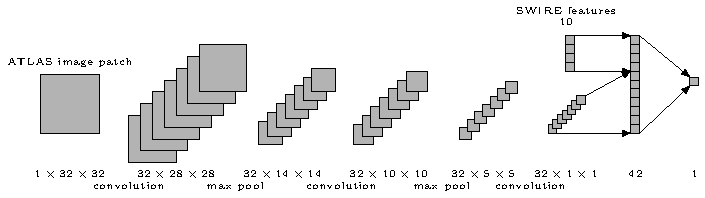
\includegraphics[width=\textwidth]{convnet.pdf}
      %   \caption{Convolutional neural network model.}
      %   \label{fig:cnn}
      % \end{figure*}

      \begin{figure}
        % \begin{tabular}{l|c}
        %   \hline
        %   Layer type & Output size\\
        %   \hline
        %   Image Input & $1 \times 32 \times 32$\\
        %   Convolution & $32 \times 28 \times 28$\\
        %   Max pooling & $32 \times 14 \times 14$\\
        %   Convolution & $32 \times 10 \times 10$\\
        %   Max pooling & $32 \times 5 \times 5$\\
        %   Dropout & $32 \times 5 \times 5$\\
        %   Merge & $810$\\
        %   Logistic regression & $1$\\
        %   \hline
        % \end{tabular}
        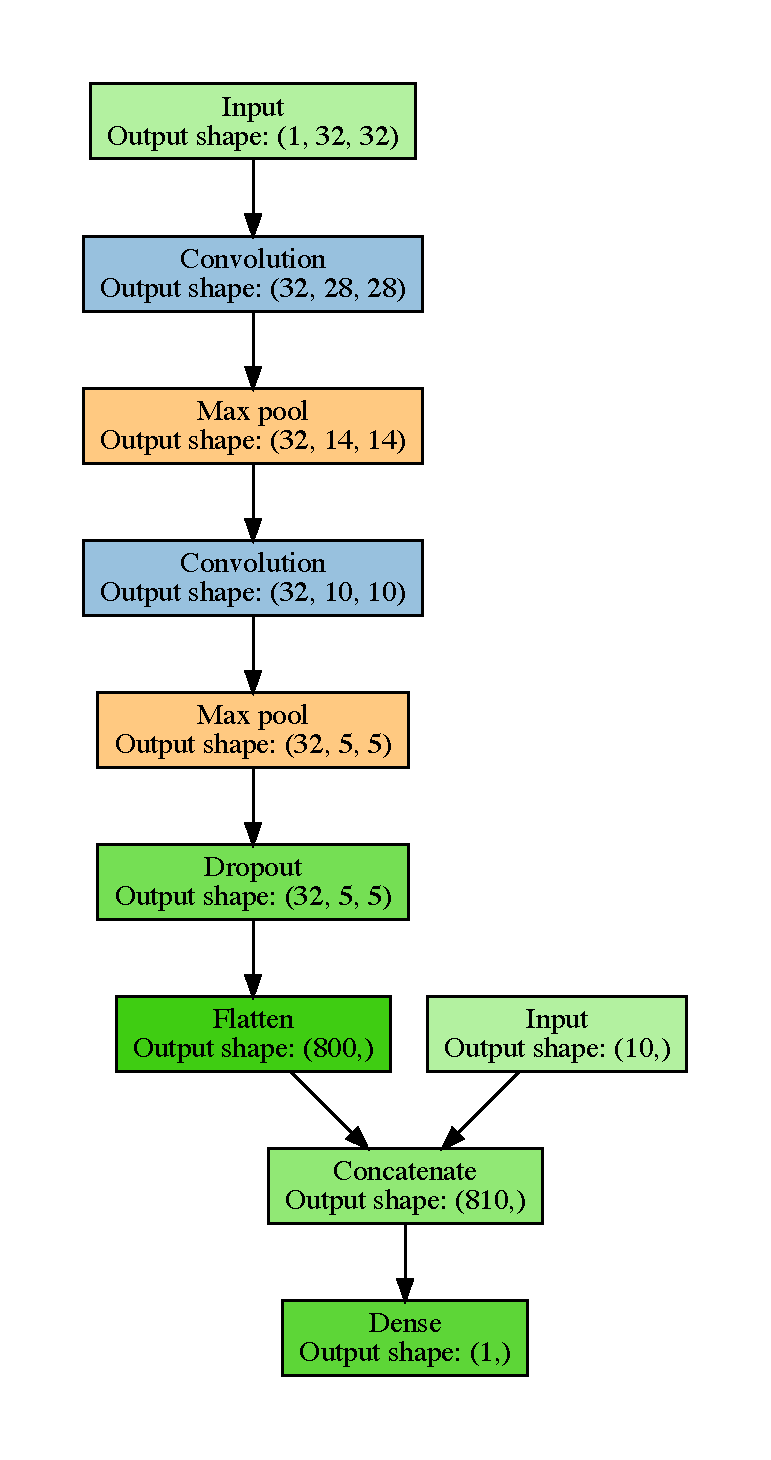
\includegraphics[width=\linewidth]{images/cnn_model_graph}
        \caption{Architecture of our CNN. The merge layer flattens the output of
          the previous layer and adds the 10 features derived from the
          candidate host in SWIRE, i.e. the flux ratios, stellarity indices,
          and distance. The dropout layer drops $25\%$ of its
          inputs. Diagram based on \url{
          https://github.com/dnouri/nolearn}.}
        \label{fig:cnn}
      \end{figure}

      % \todo{Add a diagram of convolutional filters?}

      CNNs have recently produced good results on large image-based datasets in
      astronomy \citep[e.g.][]{dieleman15cnn, lukic17compact}. We employ only a
      simple CNN model in this paper as a proof of concept that CNNs may be used
      for class probability prediction on radio images. The model architecture
      we used is shown in \autoref{fig:cnn}.

    \subsubsection{Random Forests}
    \label{sec:random-forests}

      Random forests are an ensemble of decision
      trees~\citep{breiman01random-forest}. It considers multiple subsamples
      of the training set, where each bootstrap subsample is sampled with
      replacement from the training set. For each subsample a decision tree
      classifier is constructed, which builds an axis parallel split based on
      individual features in a greedy fashion. In a random forest the split
      decision is taken based on a random subset of features. For each test
      point, the random forest takes the weighted average of all the
      classifications produced by each decision tree.

  \subsection{Labels}\label{labels}

    Converting the Radio Galaxy Zoo and \citet{norris06} cross-identification
    catalogues to binary labels for infrared objects is a non-trivial task. A
    clear problem is that there is no way to capture radio morphology
    information in binary classification. As a result, we ignore this problem
    for this paper. Another problem is that there is no way to indicate
    \emph{which} radio object an infrared object is associated with, only that
    it is associated with \emph{some} radio object. We make the na\"ive
    assumption that any given radio image contains only one host galaxy as the
    first method in solving this problem.

    We then generate positive labels from a cross-identification catalogue.
    We decide that if an infrared object is listed in the catalogue, then it
    is assigned a positive label as a host galaxy. In principle we would
    then assign every other galaxy a negative label. This has some problems
    --- an example is that if the cross-identifier did not observe a radio
    object (e.g.~it was below the signal-to-noise ratio) then the host galaxy of
    that radio object would receive a negative label. This occurs with
    \citet{norris06} cross-identifications, as these are associated with the
    first data release of ATLAS. The first data release went to a 5$\sigma$ flux
    density level of $S_{1.4} \geq 1 \text{ mJy beam}^{-1}$ \citep{norris06},
    compared to $S_{1.4} \geq \unit{85}{\micro\jansky}\text{ beam}^{-1}$ for the
    third data release used by Radio Galaxy Zoo \citep{franzen15}. The expert
    labels may therefore disagree with labels from Radio Galaxy Zoo even if they
    are both correct. We train and test our classifiers on infrared objects
    within a 1~arcmin radius of an ATLAS radio object.

  \subsection{Experimental Setup}
  \label{sec:experimental-setup}

    \begin{figure}
      \centering
      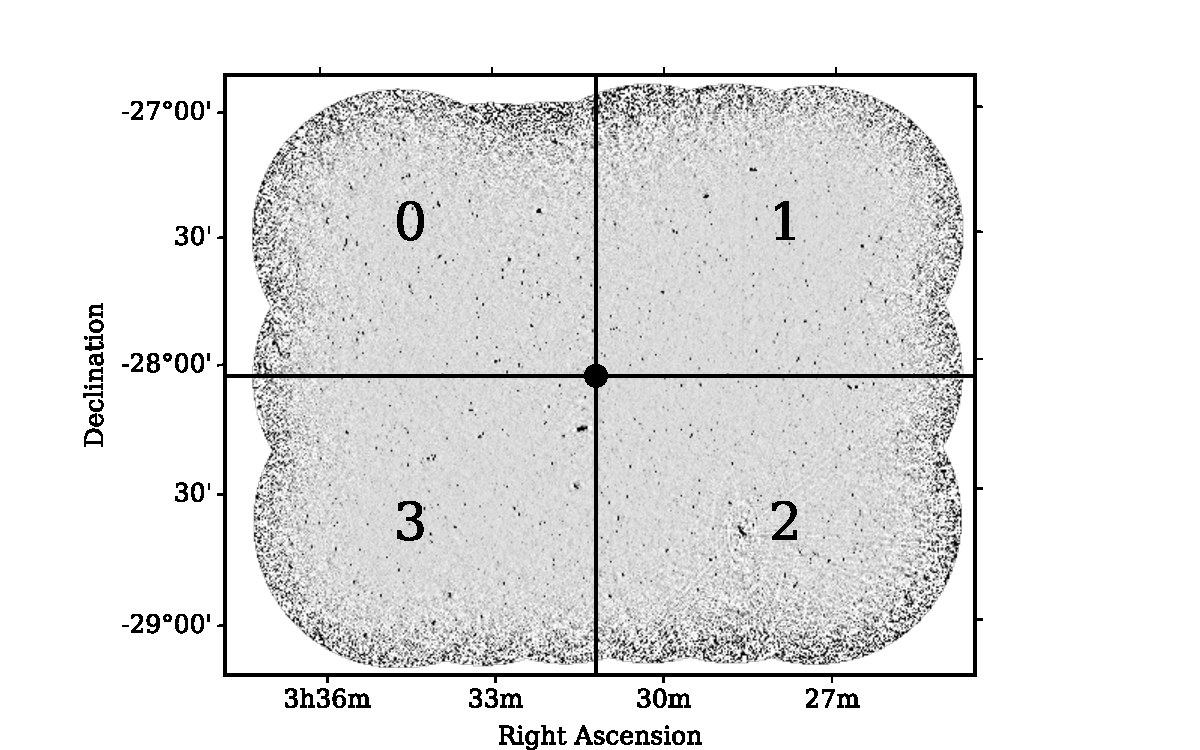
\includegraphics[width=\columnwidth]{images/quadrants.pdf}
      \caption{CDFS field training and testing quadrants labelled 0 -- 3. The
        central dot is located at $\alpha = 52^\text{h}48^\text{m}00^\text{s},
        \delta = -28^\circ{}06'00''$. The quadrants were chosen such that
        there are similar numbers of radio sources in each
        quadrant.\label{fig:quadrants}}
    \end{figure}

    We trained cross-identifiers on radio objects from the ATLAS observations of
    the CDFS field, using two label sets. One label set was derived from Radio
    Galaxy Zoo cross-identifications and the other was derived from the
    \citet{norris06} cross-identification catalogue. We refer to these as the
    Radio Galaxy Zoo labels and the expert labels respectively. We divided the
    CDFS field into four quadrants for training and testing. The quadrants were
    centred on $\alpha = 52^\text{h}48^\text{m}00^\text{s},
    \delta = -28^\circ{}06'00''$ as shown in \autoref{fig:quadrants}. For
    each trial, one quadrant was used to draw test examples and the other three
    quadrants were used for training examples.

    We further divided the radio components into compact and resolved. Compact
    components are cross-identified by fitting a 2D Gaussian \citep[as
    in][]{norris06} and we would expect any machine learning approach for host
    cross-identification to attain high accuracy on this set. Whether a
    component was resolved was decided based on its flux; a radio component was
    considered resolved if
    \begin{equation}
        \ln \left(
          \frac{S_{\text{int}}}
               {S_{\text{peak}}}
        \right) > 2\sqrt{\left(
          \frac{\sigma_{S_{\text{int}}}}
               {S_{\text{int}}}
        \right)^2 + \left(
          \frac{\sigma_{S_{\text{peak}}}}
               {S_{\text{peak}}}
        \right)^2},
    \end{equation}%
    and compact otherwise, where \(S_{\text{int}}\) is the integrated flux
    density and \(S_{\text{peak}}\) is the peak flux density
    \citep{franzen15}.

    Candidate hosts were selected from the SWIRE catalogue. For a given subset
    of radio objects, all SWIRE objects within 1~arcmin of all radio objects in
    the subset were added to the associated SWIRE subset.

    Classifiers were trained on all available training data in the training
    quadrants. Test examples were drawn from the remaining quadrant. To reduce
    bias in the testing data due to the expert labels being generated from a
    shallower data release of ATLAS, a SWIRE object was only added to the test
    set if it was within 1~arcmin of a radio object with a cross-identification
    in both the \citet{norris06} catalogue and the Radio Galaxy Zoo catalogue.

    Each classifier was trained on the training examples and used to predict
    labels for the test examples. The predicted labels were compared to the
    expert labels and the balanced accuracy was computed. We used balanced
    accuracy as our accuracy measure due to the highly imbalanced classes --- in
    our total set of SWIRE objects within 1~arcmin of an ATLAS object, only
    4~percent have positive labels. Only examples within 1~arcmin of ATLAS
    objects in the first ATLAS data release \citep{norris06} were used to
    compute accuracy, as these were the only ATLAS objects with expert labels.

    We then used the outputs of our classifiers to predict the host galaxy for
    each radio component cross-identified by both \citet{norris06} and Radio
    Galaxy Zoo. For each SWIRE object within 1~arcmin of the radio component,
    the probability of the object having a positive label was estimated using
    the trained binary classifiers. The SWIRE object with the highest
    probability was chosen as the host galaxy. The accuracy was then estimated
    by counting how many predicted host galaxies matched the \citet{norris06}
    cross-identifications.

\section{Results}\label{sec:results}

  \begin{figure}
  \centering
  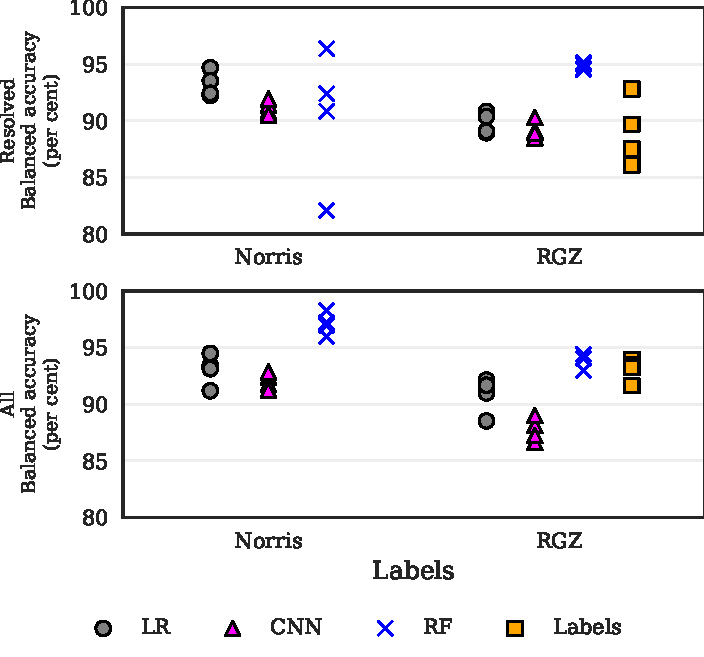
\includegraphics[width=\columnwidth]{images/cdfs_ba_grid.pdf}
  \caption{Balanced accuracies for each quadrant in the galaxy
    classification task. The accuracies of different classifiers are represented
    by different shapes. The horizontal axis shows which label set was used to
    train the classifiers: `Norris' represents the expert labels, `RGZ'
    represents the Radio Galaxy Zoo labels, and `RGZ N' represents the Radio
    Galaxy Zoo labels applied only to the radio components that appeared in the
    expert cross-identification catalogue. The three plots show different sets
    of training and testing data: the `compact' contains only compact radio
    components, `resolved' only contains resolved radio components, and `all'
    contains all radio components. The maximum attainable balanced accuracy is
    100~percent, when every galaxy label matches the expert labels.
    \label{fig:ba}}
  \end{figure}

  \begin{figure}
    \centering
    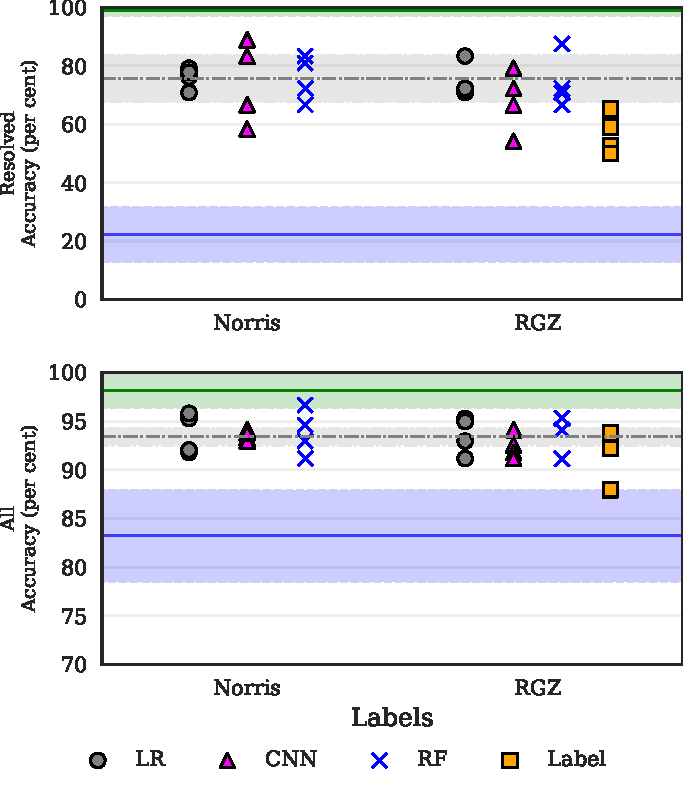
\includegraphics[width=\columnwidth]{images/cdfs_cross_identification_grid.pdf}
    \caption{Accuracies for each quadrant in the cross-identification
      task. Markers and axes are as in \autoref{fig:ba}. The upper horizontal line
      indicates the accuracy of a `perfect' classifier on the cross-identification
      task, with the surrounding dashed lines indicating the standard deviation
      across CDFS quadrants. A `perfect' classifier simply reads the expert
      labels. This represents the maximum attainable cross-identification accuracy
      under our assumptions. The lower horizontal line indicates the average
      accuracy of 15 random classifiers, and hence represents the minimum accuracy
      we would expect to attain. The surrounding dashed lines indicate the
      standard deviation across CDFS quadrants and classifiers.
      \label{fig:cross-id-accuracy}}
  \end{figure}

  The balanced accuracy of each classifier is shown in \autoref{fig:ba}. The
  best overall performance is attained by random forests trained on expert
  labels. With the exception of random forests trained only on resolved
  components, classifiers trained on expert labels on average perform better
  than those trained on Radio Galaxy Zoo labels. Nevertheless, classifiers
  trained on Radio Galaxy Zoo labels still attain reasonably good accuracies on
  all tasks. Averaging over quadrants, random forests outperform all other
  classifiers overall. When trained on resolved components and expert labels,
  the accuracy of random forests on the classification task has a very high
  spread over the CDFS quadrants. This may be due to the limited number of
  resolved components in the expert-labelled data set.

  The predicted probabilities for each SWIRE object are
  reported in \autoref{tab:probs}. Probabilities reported for a given object
  were predicted by classifiers tested on the quadrant containing that object.

  The cross-identification accuracy for each classifier is shown in
  \autoref{fig:cross-id-accuracy}. Despite relatively poor performance on the
  classification task, CNN produce good results on the cross-identification task
  when trained on the expert labels. Logistic regression gives consistent, good
  results on both expert and Radio Galaxy Zoo labels. Random forests perform
  much more poorly on the cross-identification task than on the classification
  task, possibly as they produce discrete predicted probabilities.

  The predicted cross-identification for each ATLAS object is reported in
  \autoref{tab:cids}. As with SWIRE predictions, reported cross-identifications
  for a given object were generated by classifiers tested on the quadrant
  containing that object.

  \begin{figure*}
    \subfloat[\label{fig:fail-a}]{\includegraphics[width=0.45\linewidth]{images/examples/\detokenize{CNN_Norris_ATLAS3_J032629.61-284052.7C}.pdf}}\hspace{1cm}
    \subfloat[\label{fig:fail-b}]{\includegraphics[width=0.45\linewidth]{images/examples/\detokenize{CNN_Norris_ATLAS3_J032824.66-274149.7C}.pdf}}\\
    \subfloat[\label{fig:fail-c}]{\includegraphics[width=0.45\linewidth]{images/examples/\detokenize{CNN_Norris_ATLAS3_J032908.32-284827.0C}.pdf}}\hspace{1cm}
    \subfloat[\label{fig:fail-d}]{\includegraphics[width=0.45\linewidth]{images/examples/\detokenize{CNN_Norris_ATLAS3_J032916.31-272341.2C}.pdf}}\\
    \caption{Radio sources in CDFS incorrectly cross-identified by a
      convolutional neural network trained on expert labels.
      \protect\subref{fig:fail-a}, \protect\subref{fig:fail-e}, and
      \protect\subref{fig:fail-f} have multiple SWIRE host galaxies very close
      together and the predicted host galaxy is close to the true host galaxy.
      \protect\subref{fig:fail-b} contains multiple radio sources, and the
      identified host likely \emph{is} a host galaxy, but not one labelled in
      the initial ATLAS data release, as it is a low flux source. In
      \protect\subref{fig:fail-c}, the classifier seems to be distracted by the
      right lobe of the radio source. This may be due to the large number of
      compact objects in the training set.
      \protect\subref{fig:fail-d} and \protect\subref{fig:fail-h} show the
      classifier failing to correct cross-identify a radio double. This may be
      due to the window size (both lobes would not be visible in the radio image
      shown to the classifier) or due to the limited number of radio doubles in
      the training set. Finally,
      \protect\subref{fig:fail-g} shows the classifier failing to classify a radio
      triple. This triple extends outside the 1~arcmin radius used to select
      candidate hosts.}
  \end{figure*}
  \begin{figure*}
    \setcounter{subfigure}{4}
    \subfloat[\label{fig:fail-e}]{\includegraphics[width=0.45\linewidth]{images/examples/\detokenize{CNN_Norris_ATLAS3_J033022.32-272121.1C}.pdf}}\hspace{1cm}
    \subfloat[\label{fig:fail-f}]{\includegraphics[width=0.45\linewidth]{images/examples/\detokenize{CNN_Norris_ATLAS3_J033242.02-273818.8C}.pdf}}\\
    \subfloat[\label{fig:fail-g}]{\includegraphics[width=0.45\linewidth]{images/examples/\detokenize{CNN_Norris_ATLAS3_J033433.94-271812.9C}.pdf}}\hspace{1cm}
    \subfloat[\label{fig:fail-h}]{\includegraphics[width=0.45\linewidth]{images/examples/\detokenize{CNN_Norris_ATLAS3_J033436.18-272632.0C}.pdf}}\\
    \contcaption{}
  \end{figure*}

  \begin{table}
    \caption{Average cross-identification accuracies across quadrants.
      Uncertainties represent standard deviations. `Data set' indicates whether
      the classifiers were trained and tested on resolved sources or all
      sources. `Labeller' indicates what label set the classifiers were trained
      on; `Norris' is the expert label set, `RGZ' is the Radio Galaxy Zoo label
      set, and `RGZ N' is the Radio Galaxy Zoo label set with only radio sources
      that were also labelled by experts. A `perfect' classifier reads the
      expert labels directly and hence represents the maximum attainable
      accuracy under our assumptions. A `random' classifier generates uniform
      random class probabilities and hence represents the expected minimum
      attainable accuracy with our cross-identification method. `LR' refers to
      logistic regression, `CNN' refers to our convolutional neural network, and
      `RF' refers to random forests.}
    \label{tab:cross-id-accuracies}
    \begin{tabular}{lll|l}
      \hline
      Data set & Labeller & Classifier & Mean accuracy (\%)\\
      \hline
      Resolved & Norris & Perfect & $92.06 \pm 1.46$\\
       &  & Random & $4.68 \pm 3.91$\\
       &  & LR & $66.47 \pm 6.93$\\
       &  & CNN & $61.06 \pm 15.05$\\
       &  & RF & $67.21 \pm 5.90$\\
       & RGZ N & LR & $64.63 \pm 11.10$\\
       &  & CNN & $48.61 \pm 11.54$\\
       &  & RF & $65.77 \pm 4.72$\\
       & RGZ & LR & $59.97 \pm 11.49$\\
       &  & CNN & $37.90 \pm 8.72$\\
       &  & RF & $56.99 \pm 6.13$\\
      All & Norris & Perfect & $96.74 \pm 1.76$\\
       &  & Random & $79.71 \pm 5.43$\\
       &  & LR & $92.81 \pm 1.54$\\
       &  & CNN & $92.95 \pm 1.49$\\
       &  & RF & $92.36 \pm 1.24$\\
       & RGZ N & LR & $91.73 \pm 0.95$\\
       &  & CNN & $87.55 \pm 2.13$\\
       &  & RF & $89.19 \pm 3.38$\\
       & RGZ & LR & $92.55 \pm 1.93$\\
       &  & CNN & $86.37 \pm 2.67$\\
       &  & RF & $87.12 \pm 2.58$\\
      \hline
    \end{tabular}
  \end{table}

  \cheng{Generate results and plots for accuracy, for the supplement}

  \begin{table*}
    \caption{Predicted probabilities that each object in SWIRE is a host
      galaxy. Probabilities are reported for each predictor. C(A / B) indicates
      the predictor using classifier model C, trained on label set A on data set
      B. Ellipsis indicates columns that have been omitted. The omitted columns
      are all other combinations of classifier, label set, and data set. If a
      SWIRE object does not appear in the table, then it was further than 1
      arcmin from an ATLAS object and hence has a predicted probability of zero
      by our assumptions. Full table electronic.}
    \label{tab:probs}
    \begin{tabular}{c|ccccccccccccccccccccccccccccc}
      \hline
      SWIRE & RA & Dec & CNN(Norris / All) & CNN(Norris / Compact) & \dots & RF(RGZ N / Resolved) \\
      \hline
      SWIRE3\textunderscore J032559.15-284724.2 & 51.4965 & -28.7901 & 0.0001 & 0.3585 & \dots & 0.2815 \\
      SWIRE3\textunderscore J032559.91-284728.9 & 51.4996 & -28.7914 & 0.0004 & 0.3909 & \dots & 0.0000 \\
      SWIRE3\textunderscore J032600.02-284736.9 & 51.5001 & -28.7936 & 0.0002 & 0.3395 & \dots & 0.0000 \\
      SWIRE3\textunderscore J032600.13-284637.5 & 51.5005 & -28.7771 & 0.0004 & 0.4546 & \dots & 0.0696 \\
      SWIRE3\textunderscore J032600.13-284715.7 & 51.5006 & -28.7877 & 0.0014 & 0.3857 & \dots & 0.0000 \\
      SWIRE3\textunderscore J032600.98-284705.4 & 51.5041 & -28.7848 & 0.0205 & 0.3742 & \dots & 0.0000 \\
      SWIRE3\textunderscore J032601.03-284711.6 & 51.5043 & -28.7866 & 0.0699 & 0.3752 & \dots & 0.0000 \\
      SWIRE3\textunderscore J032601.56-284131.0 & 51.5065 & -28.692 & 0.0001 & 0.3917 & \dots & 0.0819 \\
      SWIRE3\textunderscore J032601.60-284207.5 & 51.5067 & -28.7021 & 0.0000 & 0.3182 & \dots & 0.0000 \\
      \hline
    \end{tabular}
  \end{table*}

  \begin{table*}
    \small
    \caption{Predicted host galaxy cross-identifications for each object in
      ATLAS-CDFS. Cross-identifications are reported for each predictor, with
      the predictor listed as in \autoref{tab:probs}. The cross-identification
      given by \citet{norris06} is included in the `Norris' column. The
      cross-identification given by the Radio Galaxy Zoo consensus is included
      in the `RGZ' column, along with the corresponding consensus levels for
      the radio morphology and host cross-identification tasks \citep[see][for
      details on how consensus is calculated]{wong17}. Low radio consensus
      indicates that the component has multiple nearby components (and thus is
      more impacted by our assumption that the source is isolated), and low
      infrared consensus indicates that the host galaxy is unclear in the SWIRE
      image (possibly due to multiple nearby candidate host galaxies). Full
      table electronic.}
    \begin{tabular}{c|cccccccccc}
      \hline
      SWIRE & RA & Dec & Norris & RGZ & RGZ radio consensus \\
      \hline
      ATLAS3\textunderscore{}J032602.82-284708.1C & 51.511734 & -28.785575 & SWIRE3\textunderscore{}J032603.15-284708.5 & & 0.4516\\
      ATLAS3\textunderscore{}J032615.49-284629.4C & 51.564555 & -28.774847 & SWIRE3\textunderscore{}J032615.41-284630.7 & SWIRE3\textunderscore{}J032615.41-284630.7 & 0.2941\\
      ATLAS3\textunderscore{}J032615.55-280559.8C & 51.564799 & -28.099955 & SWIRE3\textunderscore{}J032615.52-280559.8 & SWIRE3\textunderscore{}J032615.52-280559.8 & 0.5625\\
      ATLAS3\textunderscore{}J032617.35-280710.2C & 51.572279 & -28.119491 & SWIRE3\textunderscore{}J032617.89-280707.2 & SWIRE3\textunderscore{}J032617.89-280707.2 & 0.4146\\
      ATLAS3\textunderscore{}J032625.13-280909.8C & 51.604711 & -28.152731 & SWIRE3\textunderscore{}J032625.19-280910.1 & SWIRE3\textunderscore{}J032625.19-280910.1 & 0.3158\\
      ATLAS3\textunderscore{}J032629.10-280650.1C & 51.621251 & -28.113924 & SWIRE3\textunderscore{}J032629.13-280650.7 & SWIRE3\textunderscore{}J032626.74-280636.7 & 0.3333\\
      ATLAS3\textunderscore{}J032629.61-284052.7C & 51.623385 & -28.681315 & SWIRE3\textunderscore{}J032629.54-284055.8 & SWIRE3\textunderscore{}J032629.54-284055.8 & 0.2676\\
      ATLAS3\textunderscore{}J032629.92-284753.5C & 51.624653 & -28.798195 & SWIRE3\textunderscore{}J032629.81-284754.4 & SWIRE3\textunderscore{}J032629.81-284754.4 & 1.0000\\
      ATLAS3\textunderscore{}J032630.66-283657.3C & 51.62777 & -28.615917 & SWIRE3\textunderscore{}J032630.64-283658.0 & SWIRE3\textunderscore{}J032628.56-283744.8 & 0.3611\\
      \hline
    \end{tabular}
    \begin{tabular}{ccccc}
      \hline
      RGZ IR consensus & CNN(Norris / All) & CNN(Norris / Compact) & \dots & RF(RGZ N / Resolved) \\
      \hline
      0.3214 & SWIRE3\textunderscore{}J032602.36-284711.5 & SWIRE3\textunderscore{}J032602.36-284711.5 & \dots & SWIRE3\textunderscore{}J032603.60-284627.4 \\
      0.8000 & SWIRE3\textunderscore{}J032615.41-284630.7 & SWIRE3\textunderscore{}J032615.41-284630.7 & \dots & SWIRE3\textunderscore{}J032615.41-284630.7 \\
      0.8333 & SWIRE3\textunderscore{}J032615.52-280559.8 & SWIRE3\textunderscore{}J032615.52-280559.8 & \dots & SWIRE3\textunderscore{}J032615.52-280559.8 \\
      1.0000 & SWIRE3\textunderscore{}J032617.89-280707.2 & SWIRE3\textunderscore{}J032617.89-280707.2 & \dots & SWIRE3\textunderscore{}J032616.86-280715.8 \\
      0.6667 & SWIRE3\textunderscore{}J032625.19-280910.1 & SWIRE3\textunderscore{}J032625.19-280910.1 & \dots & SWIRE3\textunderscore{}J032625.19-280910.1 \\
      1.0000 & SWIRE3\textunderscore{}J032629.13-280650.7 & SWIRE3\textunderscore{}J032629.13-280650.7 & \dots & SWIRE3\textunderscore{}J032629.13-280650.7 \\
      1.0000 & SWIRE3\textunderscore{}J032629.13-280650.7 & SWIRE3\textunderscore{}J032629.13-280650.7 & \dots & SWIRE3\textunderscore{}J032629.13-280650.7 \\
      0.8571 & SWIRE3\textunderscore{}J032629.81-284754.4 & SWIRE3\textunderscore{}J032629.81-284754.4 & \dots & SWIRE3\textunderscore{}J032629.81-284754.4 \\
      0.7308 & SWIRE3\textunderscore{}J032630.64-283658.0 & SWIRE3\textunderscore{}J032628.56-283744.8 & \dots & SWIRE3\textunderscore{}J032628.56-283744.8 \\
      \hline
    \end{tabular}
    \label{tab:cids}
  \end{table*}

  % \begin{figure}
  % \centering
  % 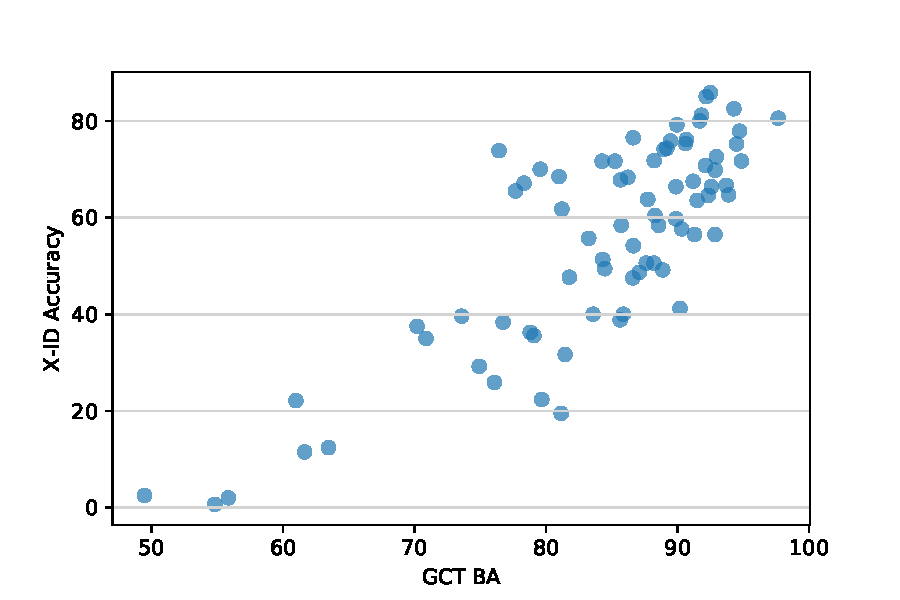
\includegraphics[width=\columnwidth]{gct-to-xid.pdf}
  % \caption{Classification balanced accuracy against accuracy on the
  % cross-identification task. Cross-identification accuracy is computed from a
  % binary comparison between the predicted host and the \citet{norris06}
  % cross-identification; neither distance to the true host nor broken assumptions
  % of one host per image are accommodated. \todo{explain this caption better
  % so that it is understandable to non-ML people; regenerate this with the new
  % pipeline}\label{fig:gct-to-xid}}
  % \end{figure}

  % \begin{figure}
  % \centering
  % 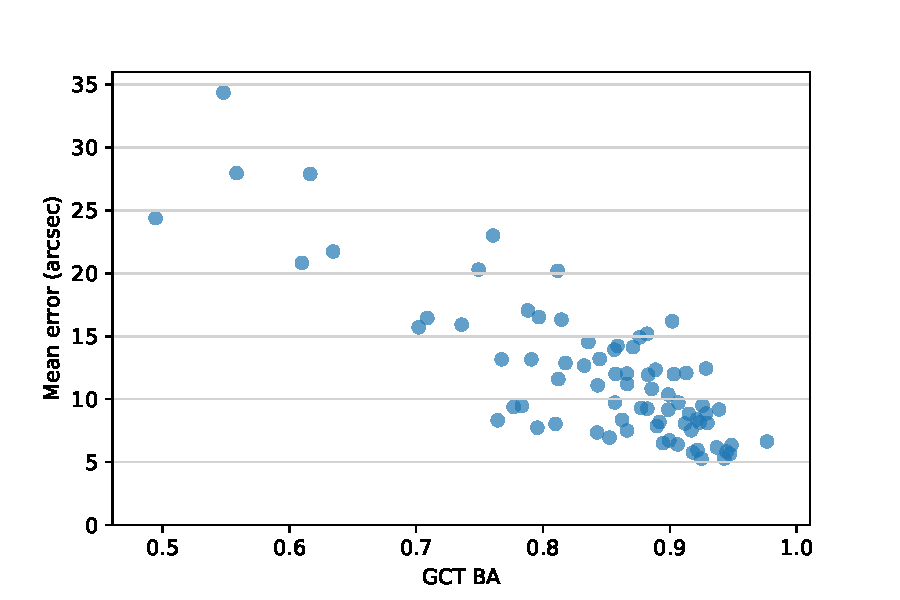
\includegraphics[width=\columnwidth]{gct-to-arcsec-error.pdf}
  % \caption{Classification balanced accuracy against average radial
  % distance between the predicted and the \citet{norris06} cross-identified
  % host on the cross-identification task.\label{fig:gct-to-arcsec-error}}
  % \end{figure}

  % \begin{figure}
  % \centering
  % 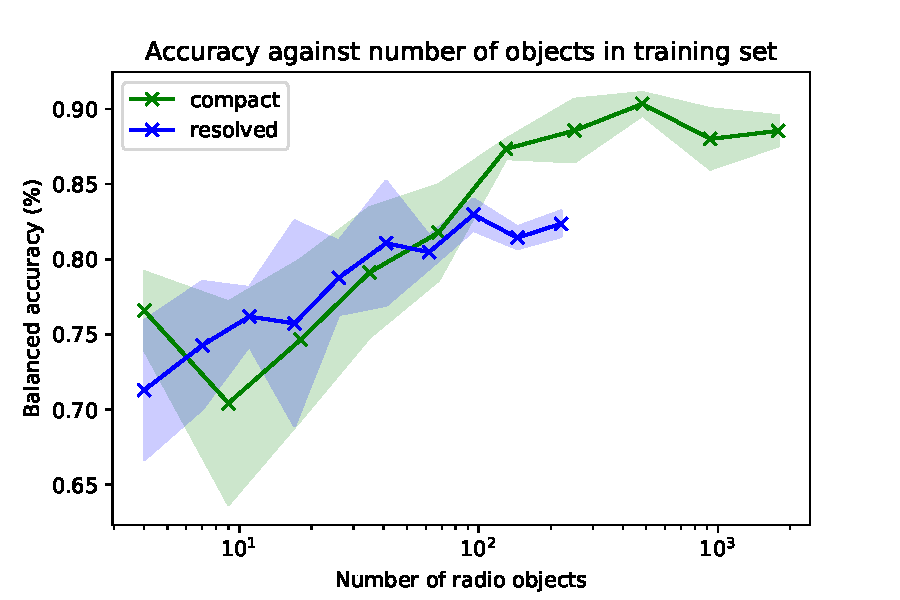
\includegraphics[width=\columnwidth]{passive.pdf}
  % \caption{Passive learning plot for the GCT. Trained and tested on RGZ.
  %   This is so that we had maximal training data --- RGZ has many more
  %   objects than Norris. \todo{Regenerate with Norris testing data}
  %   \label{fig:passive}}
  % \end{figure}

  % \begin{figure}
  % \centering
  % 
\includegraphics[width=\columnwidth]{distributions.pdf}
  % \caption{Distribution of non-image features.\label{fig:distributions}}
  % \end{figure}

  \begin{figure}
  \centering
  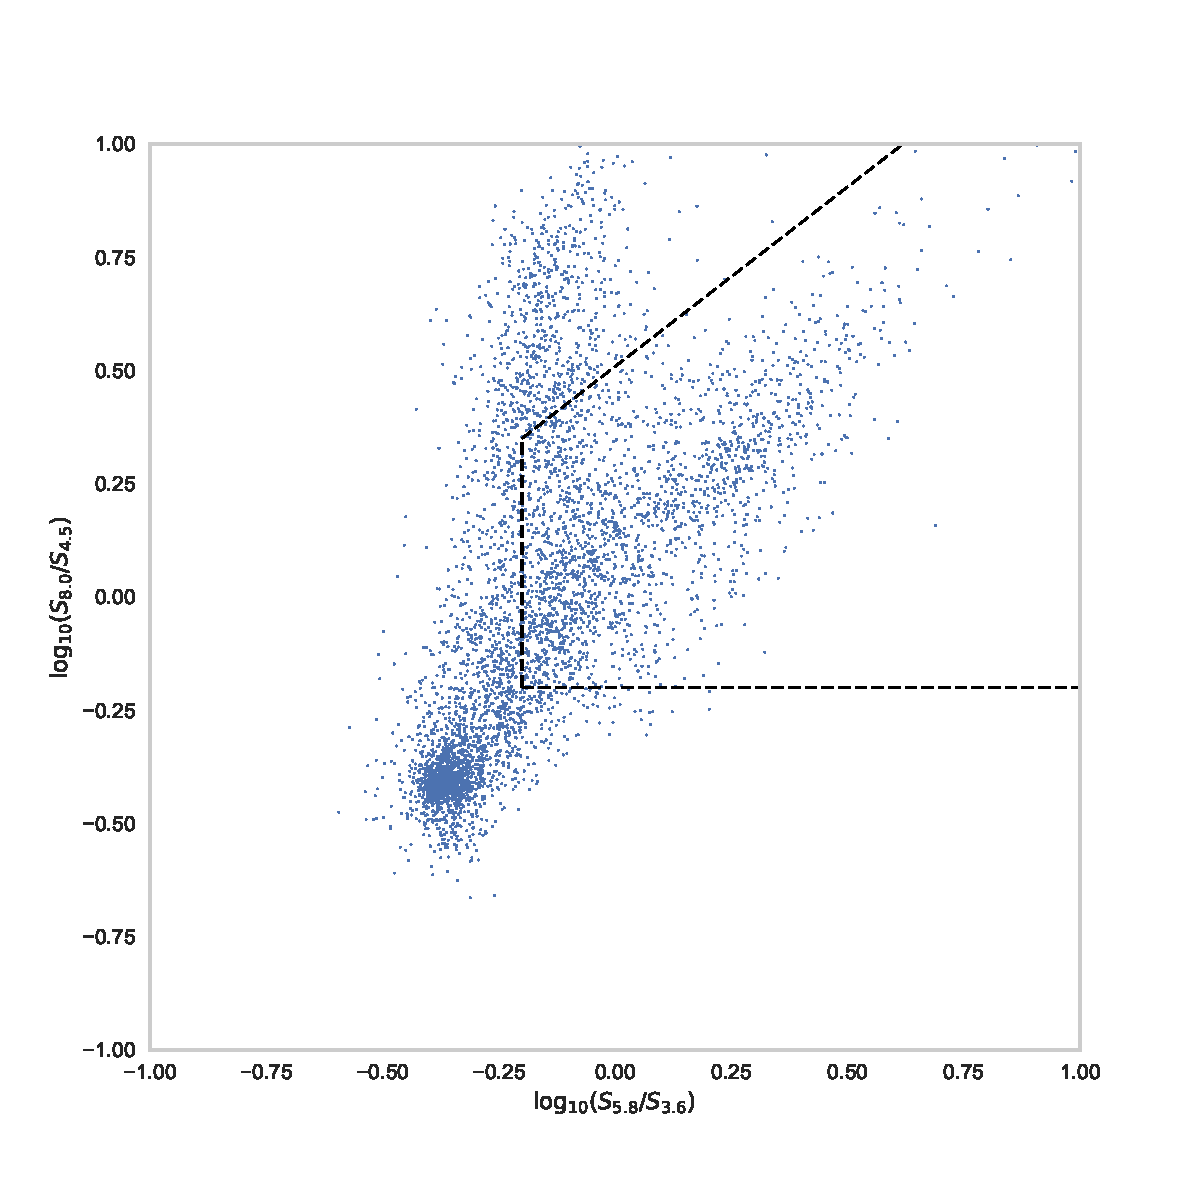
\includegraphics[width=\columnwidth]{colour-colour-all.pdf}
  \caption{Colour-colour diagram for sample of SWIRE objects within \(R\)
  of an ATLAS object.\label{fig:colour-colour-all}}
  \end{figure}

  \begin{figure}
  \centering
  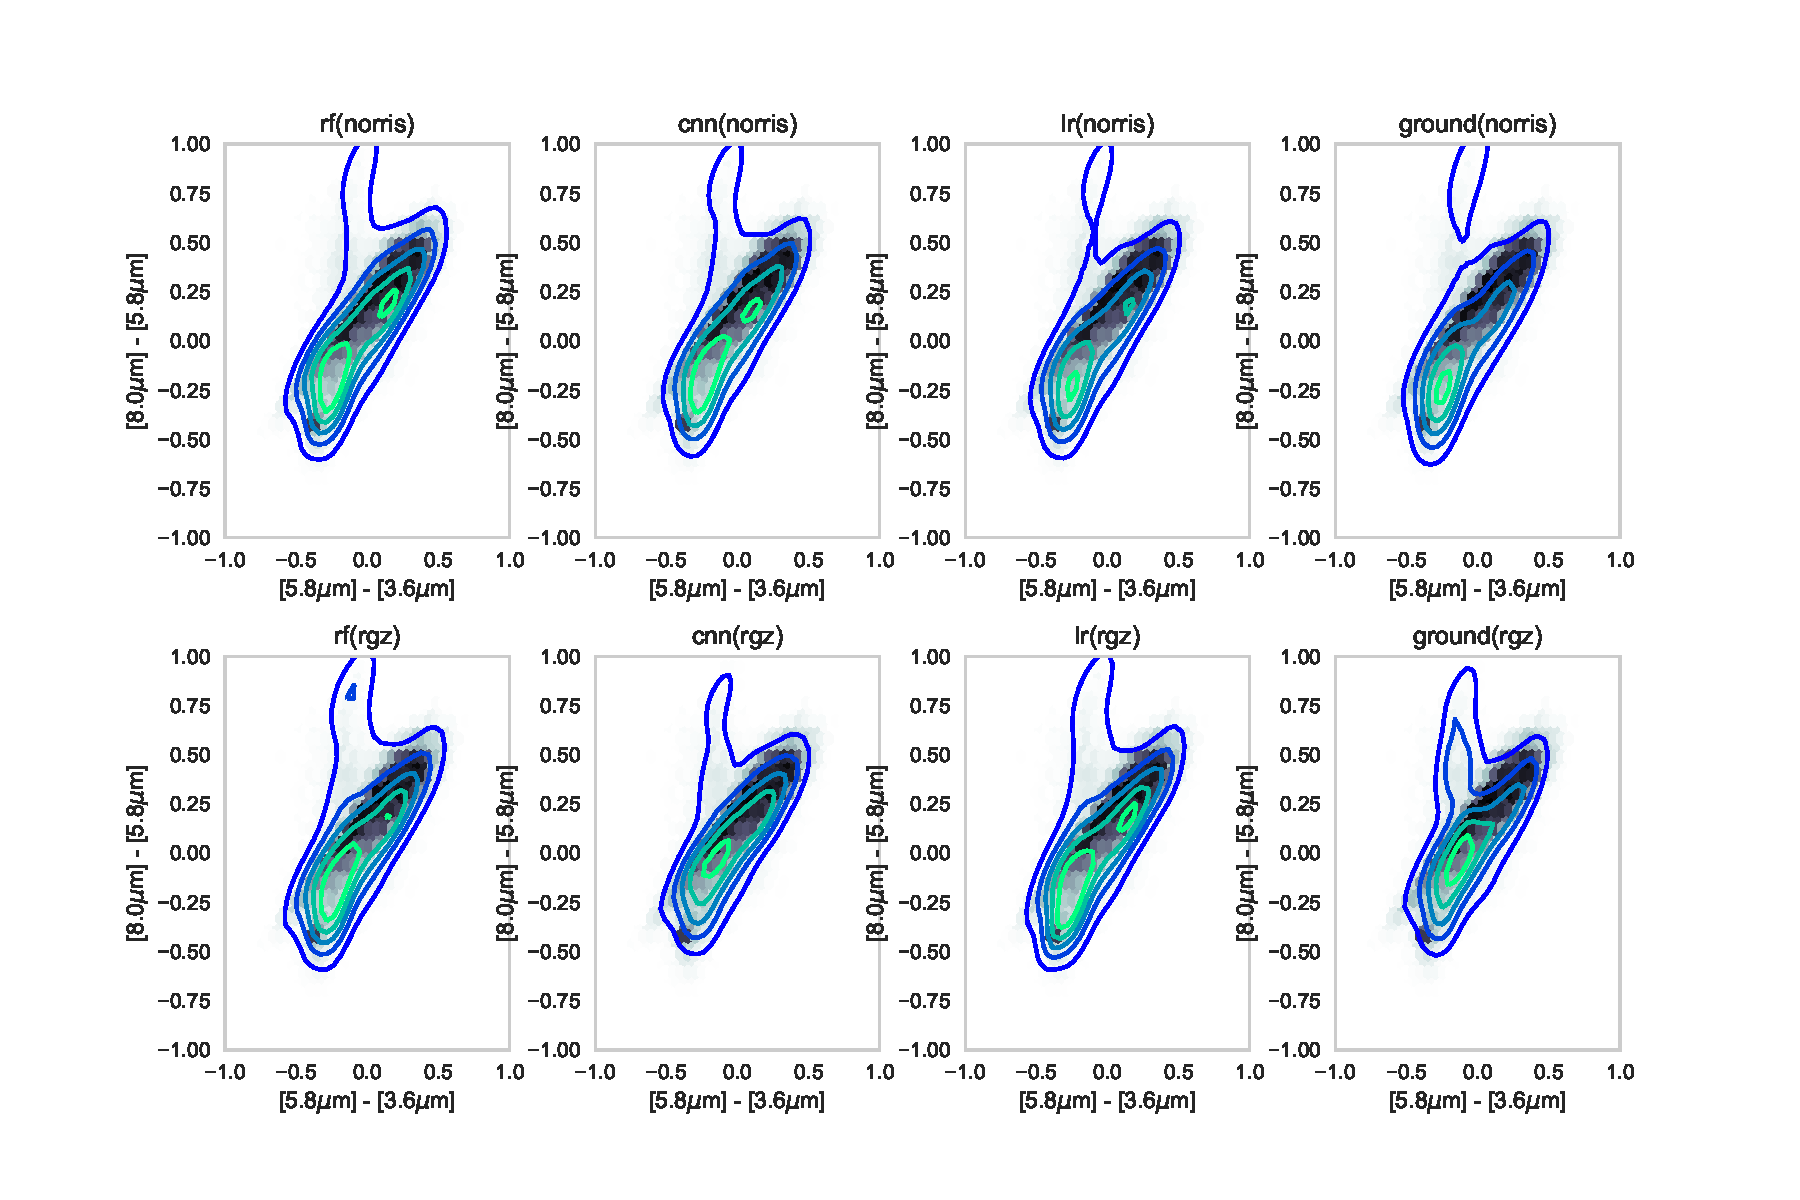
\includegraphics[width=\columnwidth]{colour_colour_predictions.pdf}
  \caption{Colour-colour diagrams for each
  classifier.\label{fig:colour-colour}}
  \end{figure}

\section{Application to ATLAS-ELAIS}
\label{sec:elais}

\section{Summary}
%
%%%%%%%%%%%%%%%%%%%% REFERENCES %%%%%%%%%%%%%%%%%%
\bibliographystyle{mnras}
\bibliography{rgz-cdfs-ms}

%%%%%%%%%%%%%%%%%%%%%%%%%%%%%%%%%%%%%%%%%%%%%%%%%%


% Don't change these lines
\bsp	% typesetting comment
\label{lastpage}
\end{document}
